\documentclass{report}
\usepackage[T1, T2A]{fontenc}% T2A for Cyrillic font encoding
\usepackage[english, russian]{babel}
\usepackage{listings}
\usepackage{mdframed}
\usepackage{csquotes}
\usepackage{graphicx}
\usepackage{stmaryrd}
\usepackage[colorlinks]{hyperref}
\usepackage{biblatex} %Imports biblatex package
\addbibresource{bible.bib} %Import the bibliography file

\lstloadlanguages{C,C++,csh,Java}
% \usepackage{mathptmx}
\usepackage{array}

\author{Сафонов Артём}
\title{Статический анализ}
\date{26.04.2025}

\begin{document}
\tableofcontents

% === #1 ===
\chapter{Анализ типов}

\section{Что будет, если в нашу систему типов ввести тип \(Bool\)?}

Продублируем изначальные правила:

\begingroup
\begin{center}
\renewcommand{\arraystretch}{1.5}
\begin{tabular}{ m{6cm} m{6cm} }
    \(I \) & \([[I]] = int\) \\
    \(E_1 == E_2 \) & \([[E_1]] == [[E_2]] \wedge [[E_1 \ op \ E_2]] = int\) \\
    \(E_1 op E_2 \) & \([[E_1]] == [[E_2]] == [[E_1 \ op \ E_2]] = int\) \\
    \(input\) & \([[input]] = int\) \\
    \(X = E\) & \([[X]] = [[E]]\) \\
    \(output \ E\) & \([[E]] = int\) \\
    \(if(E) \ \{S_1\}\) & \([[E]] = int\) \\
    \(if(E) \ \{S_1\} \ else \ \{S_2\}\) & \([[E]] = int\) \\
    \(while \ (E) \ \{S\}\) & \([[E]] = int\) \\
    \(f(X_1,...,X_n) \ \{...return \ E;\}\) & \([[f]] = ([[X_1]],...,[[X_n]]) \rightarrow [[E]]\) \\
    \((E) \ (E_1,...,E_n)\) & \([[E]] = ([[E_1]],...,[[E_n]]) \rightarrow [[(E)(E_1,...,E_n)]]\) \\
    \(\&E\) & \([[\&E]] = \&[[E]]\) \\
    \(alloc\) & \([[alloc]] = \&\alpha\) \\
    \(null\) & \([[null]] = \&\alpha\) \\
    \(^*E\) & \([[E]] = \&[[^*E]]\) \\
    \(^*X=E\) & \([[X]] = \&[[E]]\) \\
\end{tabular}
\end{center}
\endgroup

Тогда, перво-наперво введём булевый литерал в пару к \(I\) - целочисленном литералу:

\begin{center}
\(B \Rightarrow [[B]] = boolean\)
\end{center}

Понятно, что возможные значения - это \textit{True} или \textit{False}. Следовательно меняется тип выражений в инструкциях, а также у бинарных операторов - теперь стоило бы выделить логические операторы и арифметические операторы, но т.к. в TIP есть только два логических оператора то нет нужды выписывать какой-нибудь \textit{logOp}.

Ещё одно следствие - мы не знаем тип \textit{input} и \textit{output}. Выпишем изменившиеся правила:

\begingroup
\begin{center}
\renewcommand{\arraystretch}{1.5}
\begin{tabular}{ m{6cm} m{6cm} }
    \(I \) & \([[I]] = int\) \\
    \(B \) & \([[B]]] = boolean\) \\
    \(E_1 \ > \  E_2 \) & \([[E_1]] == [[E_2]] = int \wedge [[E_1 \ > \ E_2]] = boolean\) \\
    \(E_1 \ == \  E_2 \) & \([[E_1]] == [[E_2]] == [[E_1 \ == \ E_2]] = boolean\) \\
    \(E_1 \ op \ E_2 \) & \([[E_1]] == [[E_2]] == [[E_1 \ op \ E_2]] = int\) \\
    \(input\) & \([[input]] = \alpha\) \\
    \(X = E\) & \([[X]] = [[E]]\) \\
    \(output \ E\) & \([[E]] = \alpha\) \\
    \(if(E) \ \{S_1\}\) & \([[E]] = boolean\) \\
    \(if(E) \ \{S_1\} \ else \ \{S_2\}\) & \([[E]] = boolean\) \\
    \(while \ (E) \ \{S\}\) & \([[E]] = boolean\) \\
    \(f(X_1,...,X_n) \ \{...return \ E;\}\) & \([[f]] = ([[X_1]],...,[[X_n]]) \rightarrow [[E]]\) \\
    \((E) \ (E_1,...,E_n)\) & \([[E]] = ([[E_1]],...,[[E_n]]) \rightarrow [[(E)(E_1,...,E_n)]]\) \\
    \(\&E\) & \([[\&E]] = \&[[E]]\) \\
    \(alloc\) & \([[alloc]] = \&\alpha\) \\
    \(null\) & \([[null]] = \&\alpha\) \\
    \(^*E\) & \([[E]] = \&[[^*E]]\) \\
    \(^*X=E\) & \([[X]] = \&[[E]]\) \\
\end{tabular}
\end{center}
\endgroup

\subsection{Будет ли анализ более полным?}

Учитывая, что теперь в инструкциях \textit{if} и \textit{while} условие может быть только типа \textit{Bool}, следовало бы что полнота анализа увеличилась, например можно было бы найти ошибки когда в этих инструкциях условие - это арифметическое выражение, однако семантика языка не совпадает с этим правилом (в обоих инструкциях можно вставить целочисленное значение как условие), поэтому полнота всё-таки упадёт.

\subsection{Будет ли анализ более точным?}

Точность не изменится. Soundness как была такая и осталась.

\begin{quote}
   \textit{ "...if typable, then no runtime type errors occurs..." }
\end{quote}

\section{Что будет, если в нашу систему типов ввести тип \(Array\)?}

По аналогии введём литера массива, а также пустой массив:

\begin{center}
    \(\{ \; \} \Rightarrow [[\{ \; \}]] = [\alpha]\) \\
    \(\{E_1,...,E_n\} \Rightarrow \ [[E_1]] == \ ... \  == [[E2]] \) \\
    \(\ E = \{E_1,...,E_n\} \Rightarrow \ [[E]] == [ \ [[E_1]] \ ] \)
\end{center}

Все элементы массива долнжы иметь один тип, а вообще-то то есть это либо \textit{int} либо \textit{unit} (пустой массив), либо также массив, обозначим тип массива как \([<typename>] \).

\subsection{Придумайте правила вывода для новых операторов}
Введём операцию взятия индекса:

\begin{center}
    \( E[E_1] \Rightarrow [[E]] == [\alpha] \ \wedge \ [[E_1]] == int \ \wedge \ [[ \ E[E_1]\  ]] = \alpha\) \\
    \( E[E_1] = E_2 \Rightarrow [[E]] == [\alpha] \ \wedge \ [[E_1]] == int \ \wedge \ [[ \ E[E_1] \ ]] == [[E_2]] \  \wedge \ E_2 = \alpha\) \\
\end{center}

Индексация происходит по числу, следовательно тип индекса - это \textit{int}, также тип присваемого значения должен соответсвовать типу элемента массива, говоря иначе типу выражения, которое возвращает операция взятия индекса.

\newpage
\subsection{Попробуйте протипизировать программу}

Используя добавленые правила протипизируем программму:

\begingroup
\begin{center}
\begin{lstlisting}
main() {
    var x,y,z,t;
    x = {2,4,8,16,32,64};   [[x]]=[ [[2]] ]=[ int ]

    y = x[x[3]];            [[3]]=int^x=[int]=>[[x[3]]]=int=>[[x[x[3]]]]=int
                                =>[[y]]=int

    z = {{},x};             [[{}]]=[a]^[[x]]=[int]=>[[z]]= [[int]]

    t = z[1];               [[z]]=[[int]]^[[1]]=int=>[[t]]=[int]

    t[2] = y;               [[y]]=int^[[2]]=int^[[t]]=[int]=>[[t[2]]]=int
}
\end{lstlisting}
% \renewcommand{\arraystretch}{1.5}
% \begin{tabular}{ m{6cm} m{6cm} }
%     var x,y,z,t; & a \\
%     x = {2,4,8,16,32,64}; & a \\
%     y = x[x[3]]; & a \\
%     z = {{},x}; & a \\
%     t = z[1]; & a \\
%     t[2] = y; & a \\
% \end{tabular}
\end{center}
\endgroup

В результате получаем:

\begin{center}
    \( [[x]] = [\ int\ ] \) \\
    \(  [[y]] = int \) \\
    \(  [[z]] = [\ [\ int\ ]\ ] \) \\
    \(  [[t]] = int \) \\
\end{center}

\section{Дополнительные задания}

\begin{mdframed}
\textbf{Exercise 3.9, p. 24}: This exercise demonstrates the importance of the term equality
axiom. First explain what the following TIP code does when it is executed:

\begin{center}
\begin{lstlisting}
var x,y;
x = alloc 1;
y = alloc (alloc 2);
x = y;
\end{lstlisting}
\end{center}

Then generate the type constraints for the code, and apply the unification
algorithm (by hand).

\end{mdframed}

\textbf{Что делает этот код}:
\begin{enumerate}
    \item Объявляет две перемеенные Х и Й
    \item Аллоцирует ячейку памяти со значением 1 (Х - поинтер)
    \item Аллоцирует ячейку памяти со значением аллокации ячейки памяти со значением 2, иначе говоря Й - это птр на птр со значением 2
    \item Х приравнивается к Й \( \rightarrow\) икс теперь хранит ссылку на п.3
\end{enumerate}

\textbf{Протипизируем программу:}
\begin{center}
\begin{lstlisting}
var x,y;                //
x = alloc 1;            // [[x]] = [[alloc 1]]
y = alloc (alloc 2);    // [[y]] = [[alloc [[alloc 2]] ]]
x = y;                  // [[x]] = [[y]]
\end{lstlisting}
\end{center}

Получаем:
\begin{center}
\begin{lstlisting}
[[x]] = &int
[[y]] = &&int
[[x]] /= [[y]]
\end{lstlisting}
\end{center}

\section{Результат реализации TypeAnalysis в TIP}

Тестировал на программе:
\begin{lstlisting}
g(a){
    return *a;
}

f(){
    var a;
    var b;
    a=10;
    if( a == 10 ){
        b=g(&a);
    }

    return a;
}
\end{lstlisting}

Вывод анализа:
\begin{figure}
    \centering
    \includegraphics[scale=0.6]{image.png}
    \caption{Результат TypeAnalysis}
    \label{fig:enter-label}
\end{figure}

% === #2 ===
\chapter{Теория решёток}

\section{Почему нам не подходит конкретный домен?}
Для начала я обратился к \cite{Bydge06} чтобы понять вообще разницу между абстрактным и конкретным доменами (пусть и кажется оно интуитивным). Там приводится пример \textit{complete lattice}, которую называюь \textit{concrete semantic domain}. Используется анализ множества возможных состояний программы, имея такую решётку и функции трансформации можно теоритически вывести все `контексты`, возможные состояния программы, однако это было бы просто невычислимо, учитывая точность такого анализа.

Если бы нам хотелось использовать конкретный домен для определения знака в выражении, тогда мы могли бы выбрать например домен целых чисел. Тогда необходимо было бы знать конкретное значение числа для переменной, что конечно делает анализ бесконечно сложным в теории.

\section{У решетки есть максимальный и минимальный элементы...}

\subsection{Являются ли они точной верхней или нижней гранью какого-либо
подмножества S?}

Да! Доказать это можно через следующие определения \cite{StanCS353}:

\begin{quote}
A \textit{semilattice} is a partial order $(X, \leq)$ in which every doubleton $\{x, y\}$ has a least upper bound, denoted $x \vee y$ and called the \textit{join} of $x$ and $y$. Even though the relation $\leq$ is partial (i.e., not linear as an order), the operation $\vee$ is total ($x \vee y$ is well-defined for all elements $x, y \in X$).
\end{quote}

\begin{quote}
    With this definition there is a dual notion, that of lower semilattice (so “semilattice” in the above means “upper semilattice”), in which every doubleton has a greatest lower bound, denoted x $\wedge$ y and called their \textit{meet}.
\end{quote}

Определение решётки затем складывается из нижней полурешётки и верхней полурешётки:

\begin{quote}
A \textit{lattice} is a poset that is simultaneously an \textit{upper semilattice} and a \textit{lower semilattice.}
\end{quote}

Для \textit{upper semilattice} и \textit{lower semilattice} определены \(join\) и \( meet\), следовательно они присущи и решётке.

Из чего можно сделать вывод: решётка всегда имеет как точную верхнюю грань, так и точную нижнюю грань для любого конечного подмножества $S$, поскольку операции \(join\) и \( meet\) определены для всех пар элементов. Максимальный элемент решётки является точной верхней гранью всего множества, а минимальный — его точной нижней гранью.

\subsection{Уникальны ли они?}

\textit{Least upper bound} и \textit{greatest lower bound} решётки должны быть уникальны, но просто \textit{upper bound} и \textit{lower bound} для каких-либо \{a, b\} не обязаны быть уникальными.

\section{Произведения решёток}

\subsection{Как выглядит $\sqcup$ и $\sqcap$ для $L_1 \times L_2 \times . . . \times L_n$?}

Напомню сам себе определения:
\begin{itemize}
    \item $\sqcup \space L$ -
        $X \sqsubseteq \bigsqcup X \space \vee \space \forall y \in S : X \sqsubseteq y \Rightarrow \bigsqcup X \sqsubseteq y$

    \item $\sqcap \space L$ -
        $ \bigsqcap X \sqsubseteq  X \space \vee \space \forall y \in S : y \sqsubseteq X \Rightarrow  y \sqsubseteq \bigsqcap X $
\end{itemize}

Достаточно посмотреть на получившуюся после перемножения решётку:

\begin{figure}[h]
    \centering
    \includegraphics[width=0.5\linewidth]{lattice_product.png}
    \caption{Перемножение решёток}
    \label{fig:latproduct}
\end{figure}

На ней и видно, что операции $\sqcup$ и $\sqcap$ определяются \textit{покоординатно} следующим образом:

$$
(a_1, a_2, \dots, a_n) \sqcup (b_1, b_2, \dots, b_n) = (a_1 \sqcup b_1,\; a_2 \sqcup b_2,\; \dots,\; a_n \sqcup b_n)
$$
$$
(a_1, a_2, \dots, a_n) \sqcap (b_1, b_2, \dots, b_n) = (a_1 \sqcap b_1,\; a_2 \sqcap b_2,\; \dots,\; a_n \sqcap b_n)
$$

А $\top$ и $\bot$ - для $product \space L$ - кортеж из получившихся $\top$ и $\bot$

\subsection{Какая высота у произведения решеток $L_1 \times L_2 \times . . . \times L_n$?}

\[
{height}(L_1 \times \dots \times L_n) =
{height}(L_1) + \dots + {height}(L_n)
\]

\section{Точная верхняя/нижняя грань решётки отображений}

Пусть $ f $ — функция отображения. Тогда:

$$
f_\top(x) = \top \space \forall x \in A,
$$
$$
f_\bot(x) = \bot \space \forall x \in A.
$$

Эти отображения являются соответственно наибольшим и наименьшим элементами решётки отображений $ A \to L $.

\section{Высота решётки отображений}

Высота решётки отображений $ A \to L $ выражается через мощность области определения $ A $ и высоту базовой решётки $ L $:

$$
{height}(A \to L) = |A| \cdot{height}(L).
$$

\section{Почему нельзя использовать унификационный решатель?}

Потому что нам интересны уравнения вида:
$$
x_n \sqsubseteq f_n(x_1, x_2, ..., x_n)
$$

Нам интересно чтобы результат в каждоый ноде был меньше чем соотв. функция в которую мы его передали.
Для такого унификационные солверы не подходят, потому что много \textit{ambiguity}

\section{Результат реализации SignAnalysis в TIP}

Тестил над файлом:
\begin{lstlisting}
fun(x) {
    var y;
    var k ;
    k = 8;
    y = 7;
    while(k > y) {
        k = k - 1;
    }
    return 0;
}
main() {
    var pos, neg, top, zero;
    var later;
    pos = 5 + 5;
    pos = 5 * 5;
    neg = -5 - 5;
    neg = -5 * 5;
    neg = 5 * -5;
    top = 5 - 5;
    top = top * 5;
    zero = top * 0;
    zero = 5 * zero;
    later = 7;
    return 0;
}
\end{lstlisting}

Вывод в виде графа:

\begin{figure}
    \centering
    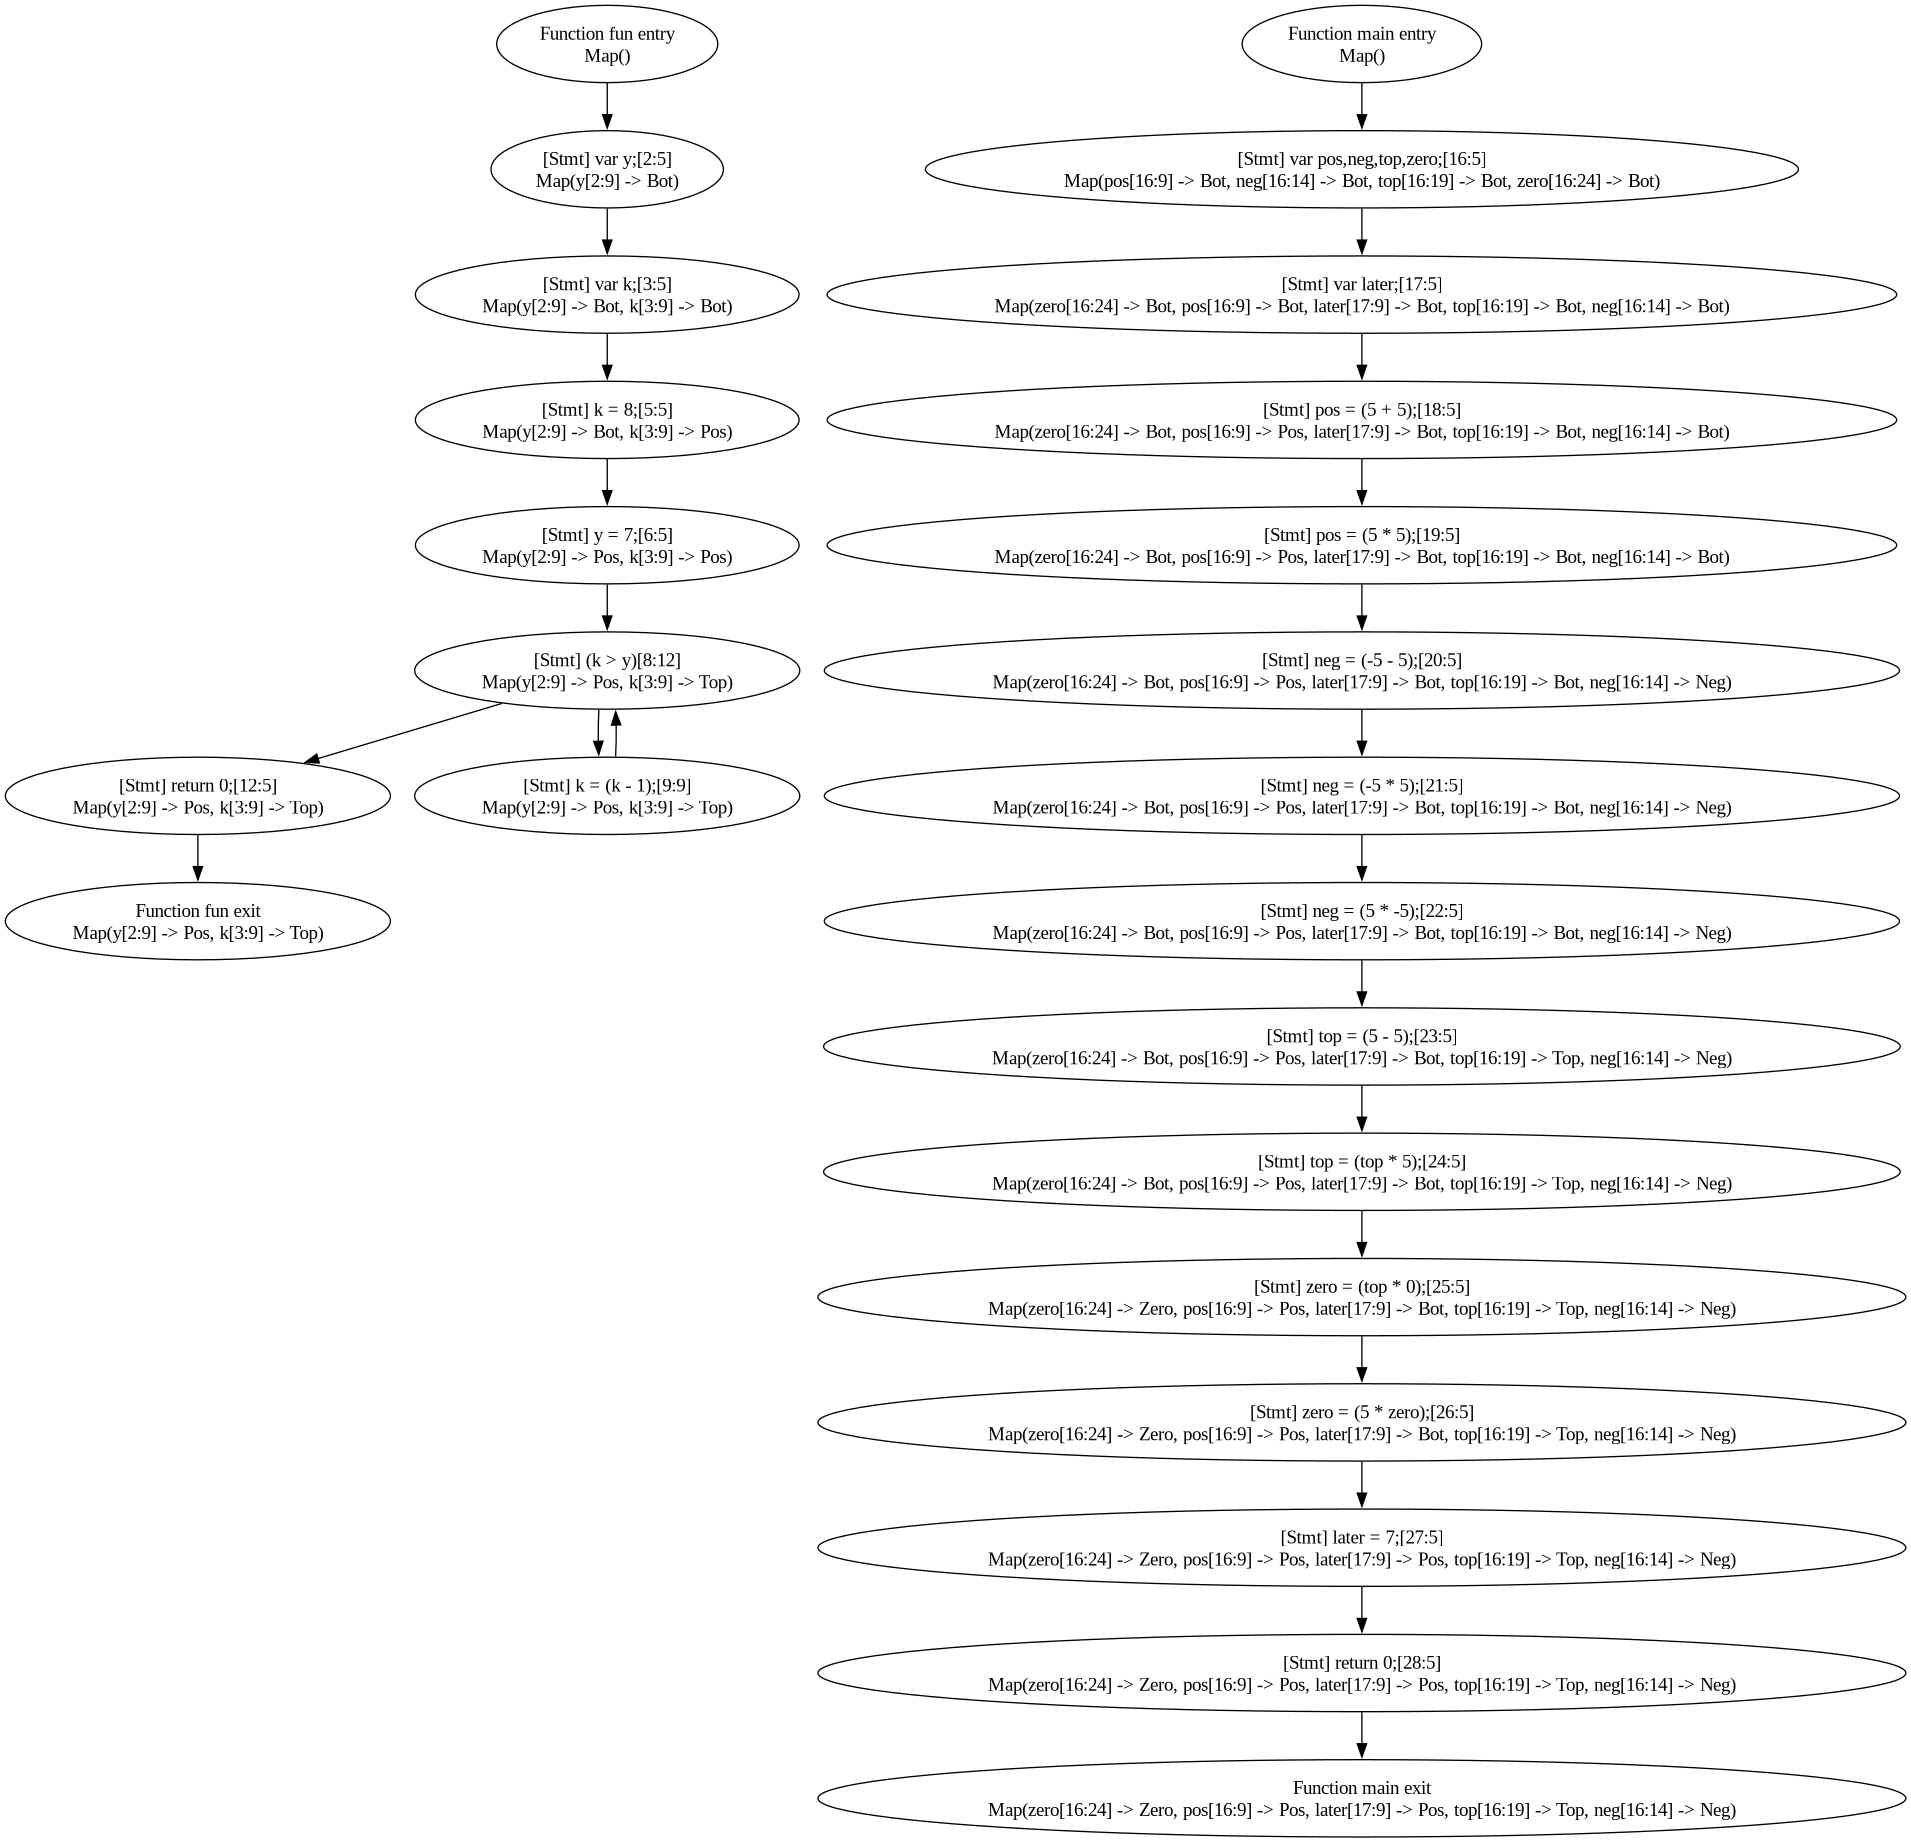
\includegraphics[scale=0.2]{signs.png}
    \caption{Резульат SignAnalysis}
    \label{fig:hi}
\end{figure}

% % === #REF ===
% \chapter{Литература}

% В процессе ответов на вопросы, да и в целом изучения курса я пользовался следующими материалами:
\printbibliography




% === #3 === %
\chapter{Потокочувствительные анализы}

\section{Какова сложность структурного алгоритма?}

Пусть $ n $ — количество узлов CFG. Алгоритм последовательно обходит все узлы графа, и для каждого из них выполняет операции добавления или удаления информации о переменных. Каждая такая операция занимает время $ O(k) $, где $ k $ — количество переменных в программе (или высота решётки, если говорить точнее).

Ппри изменении состояния узла он может быть снова добавлен в \textit{worklist} для пересчёта зависимых узлов. В худшем случае это приведёт к $ k $ проходам по всем $ n $ узлам графа — именно столько шагов нужно, чтобы достичь фикспоинта для всех переменных.

Таким образом, временная сложность алгоритма составляет:
$$
O(n \times k^2)
$$

Если в графе нет циклов (то есть, CFG ацикличен), то каждый узел обрабатывается только один раз. Это исключает повторные проходы по графу, и временная сложность снижается до:
$$
O(n \times k)
$$

Что касается сложности по памяти: нам нужно хранить состояние (значения переменных) для каждого узла программы. Общая память, таким образом, составляет:
$$
n \times k
$$
т.к. для каждого из $ n $ узлов хранится информация о $ k $ переменных.

\section{Решите систему ограничений}

Операции для \textit{very busy analysis}:
$$
[[x = E]] = removerefs(JOIN(n), x) \space \cup \space exprs(n)
$$

$[[n]] = JOIN(n) \space \cup \space exprs(n) $ - для любых других $n$

$$JOIN(v) = \bigcap_{w \in succ(v)} [[w]] $$

\textbf{Пример}:
\begin{lstlisting}
1    var x, a, b;
2    x = input;
3    a = x - 1;
4    b = x - 2;
5    while(x > 0) {
6        output a*b -x;
7        x = x - 1
8    }
9   output a*b
\end{lstlisting}

\textbf{Результат}:
\begin{lstlisting}
1 {}
3 {x-1}
4 {x-1, x-2}
5 {x-1, x-2, x > 0}
6 {a*b-x, a*b, x-1, x-2, x > 0}
7 {a*b, x-1}
9 {a*b, x-1}
\end{lstlisting}

\section{Результат реализации Live Variables Analysis}

Тестировал на:
\begin{lstlisting}
main() {
  var a,b,i;
  a = 5;
  b = 42;
  i = a;
  while (b > i) {
    // ...
    i = i + 1;
  }
  return 0;
}
\end{lstlisting}

Вывод:
\begin{figure}
    \centering
    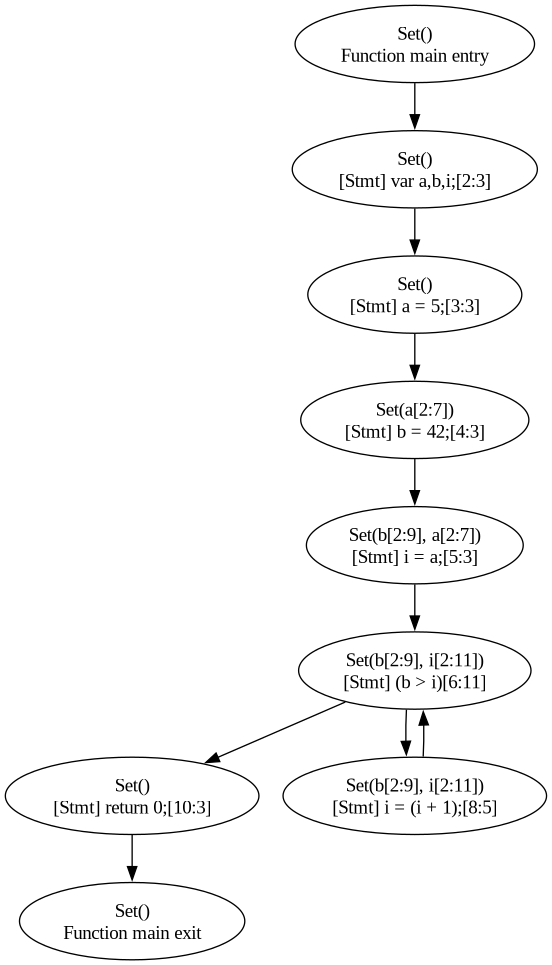
\includegraphics[width=0.5\linewidth]{loop_livevars.png}
    \caption{Результат Live Vars Analysis}
    \label{fig:enter-label}
\end{figure}

\section{Результат реализации Reaching Definitions Analysis}

Тестил на программе со слайда:
\begin{lstlisting}
main() {
    var x, y, z;
    x = input;
    while(x > 1) {
        y = x / 2;
        if (y > 3) x = x - y;
        z = x - 4;
        if (z > 0) x = x / 2;
        z = z - 1;
    }
    output x;
}
\end{lstlisting}

Вывод:
\begin{figure}
    \centering
    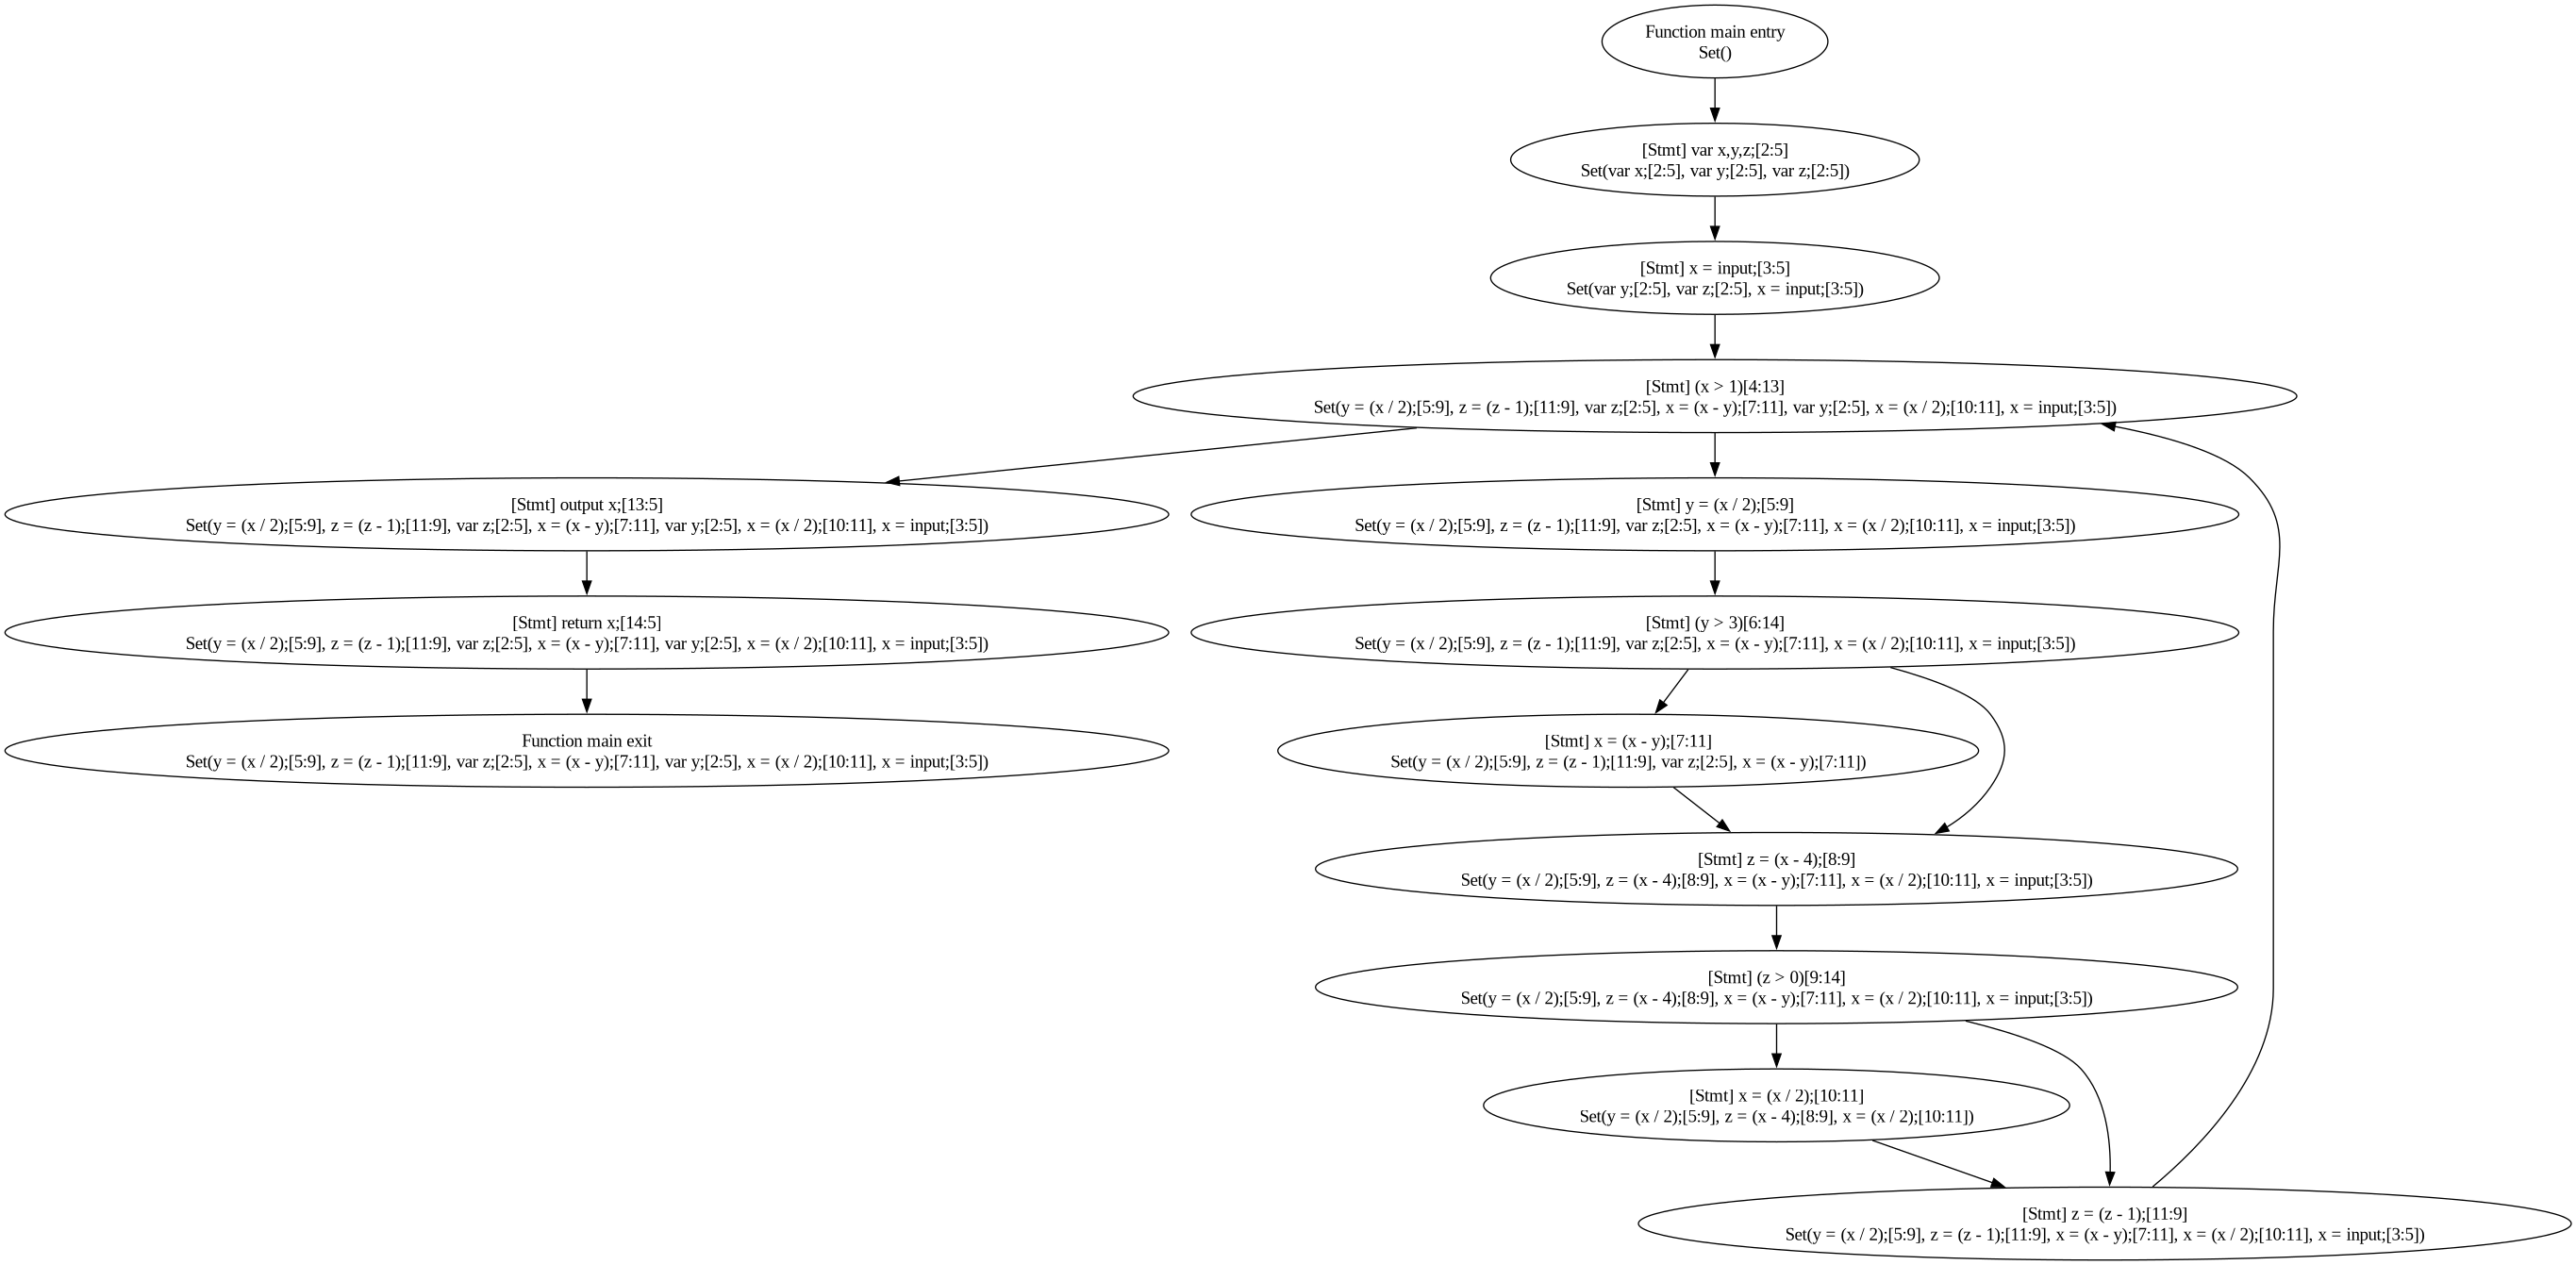
\includegraphics[width=1.4\linewidth]{reaching.png}
    \caption{Результат RD Analysis}
    \label{fig:enter-label}
\end{figure}

\end{document}